\documentclass[acmsmall,screen,review,anonymous]{acmart}

%%
%% \BibTeX command to typeset BibTeX logo in the docs
\AtBeginDocument{%
  \providecommand\BibTeX{{%
    Bib\TeX}}}

%% Rights management information.  This information is sent to you
%% when you complete the rights form.  These commands have SAMPLE
%% values in them; it is your responsibility as an author to replace
%% the commands and values with those provided to you when you
%% complete the rights form.
\setcopyright{acmcopyright}
\copyrightyear{2018}
\acmYear{2018}
\acmDOI{XXXXXXX.XXXXXXX}


%%
%% Submission ID.
%% Use this when submitting an article to a sponsored event. You'll
%% receive a unique submission ID from the organizers
%% of the event, and this ID should be used as the parameter to this command.
%%\acmSubmissionID{123-A56-BU3}

\usepackage{xcolor}
\usepackage{listings}
\usepackage{caption}
\usepackage{subcaption}

\definecolor{backcolor}{rgb}{0.95,0.95,0.92}

\lstdefinestyle{mystyle}{
  basicstyle=\ttfamily\footnotesize,
  keywordstyle=\color{blue},
  stringstyle=\color{red},
  commentstyle=\color{green},
  breakatwhitespace=true,
  breaklines=true,
  keepspaces=true,
  showspaces=false,
  showstringspaces=false,
  showtabs=false,
  tabsize=4,
  captionpos=b,
  numbers=left,
  numberstyle=\tiny\color{gray},
  backgroundcolor=\color{backcolor},
}
\lstset{style=mystyle}
\usepackage{graphicx}
\usepackage{caption}

\begin{document}

\title{Bridging the Gap Between Visual and Analytical Machine Learning Testing}

\author{Anon}

\begin{abstract}
% what is the problem?
% why is this an important problem to solve?
% what did we do?
% what did we find?
Testing ML systems is a highly interactive process which demands a human-in-the-loop approach. In addition to writing tests for the code base, practitioners are required to analyse and interpret several visualisations using their domain expertise to validate if an ML system satisfies the required set of functional and non-functional properties. Visualisations are frequently used to qualitatively assess various parts of an ML pipeline. However, implicit knowledge gained from visualisations must be translated to explicit analytical tests that fail when there is change in any component of the ML pipeline. We conduct an empirical analysis of Jupyter notebooks to catalogue the state-of-the-art mappings between ML visualisations and assertions. We mine Github to collect Jupyter Notebooks that contain assertions written in Python. We develop a novel methodology to identify 1764 notebooks which contain an assertion below a visualisation. We manually analyse the 1.7K notebooks and identify 551 notebooks where at least one pair of visualisation and assertion are semantically related to one another. We further read and understand 90 notebooks in depth to identify 26 qualitative and their corresponding quantitative testing patterns. We showcase five such patterns in this paper and plan to make the entire catalogue publicly available in the near future.

\end{abstract}

\maketitle

\section{Introduction}\label{sec:intro}
Artificial Intelligence (AI) is here to stay. Recent years show a shift from chasing high correctness of ML models to ensuring that they are safe for application in safety-critical domains such as healthcare, finance and autonomous driving. With the advent of Large Language Models, the power of AI to directly influence the daily lives of humans is growing at a radical pace. As reports of "hallucinated" facts, racist predicts and autonomous car crashes steadily increase, ensuring that ML systems function as they were intended to, takes precedence.

Visualisations are used throughout the ML development lifecycle. In the early stages of the ML development lifecycle, visualisations are extensively used for make sense of the data and understanding its statistical properties. During the model development phase, visualisations are used to summarise various metrics and summary statistics of the model's performance. Once the model is deployed in production, visualisations are used to continually monitor their performance and trigger a new training cycle once their performance drops below a certain threshold.

The research questions along with the contributions of this paper are as follows.
\begin{description}
\item[RQ1.] How frequently do ML practitioners formulate analytical tests from the visualisations they create to test ML systems?

We mine 54K Jupyter notebooks from Github that contain an assertion written in Python. We develop a novel technique to identify 1764 notebooks which an assertion below a visualisation. We manually analyse the 1.7K notebooks and identify 551 notebooks that contain at least one pair of visualisation and assertion that are semantically related to each other.

\item[RQ2.] What are the types of visualisation and assertion pairs typically used by ML practitioners when testing ML systems?

From the 553 notebooks, we further perform an in-depth analyse of 90 notebooks. We identify 26 unique visualisation and assertion pairs. We discuss five such pairs in this paper and plan to release the full catalogue publicly in the near future.

\end{description}

This paper is organised as follows...

\section{Preliminaries}\label{sec:prelim}

\subsection{ML Testing}\label{sec:ml-testing}

Testing ML enabled software systems poses more challenges compared to their traditional counter part. While traditional software systems mature through change in their codebase, ML enabled systems experience change in the training data and the machine learning model in addition to the codebase. With ML being adopted into safety-critical domains that can affect human lives, ensuring that ML systems are correct, robust to data perturbations and not biased by race, colour and gender is of paramount importance. Existing scientific literature on ML testing broadly focuses on two aspects. First, the functional property of correctness of the model in making predictions for previously unseen data. And the non-functional property of fairness towards humans of different race, colour, gender, sexual orientation and disabilities.

% TODO verify that the papers cited are actually on test adequacy metrics
To test the correctness of ML models, several improvements over existing test adequacy metrics have been proposed. Tools such as \textit{DeepExplore} and \textit{DeepGauge} propose new test adequacy metrics such as neuron coverage adapted for ML enabled software systems~\cite{pei2017deepexplore, ma2018deepgauge, gerasimou2020importance}. Formal verification methods have also been proposed that try to provide formal guarantee of robustness against adversarial examples. Such methods however are only feasible for statistical ML models and become computationally expensive for more complex models such as deep neural networks~\cite{zhu2021deepmemory, baluta2021scalable}. Several works have been conducted on generating and detecting adversarial inputs for ML models. Data augmentation techniques based on fuzzing, search based software testing and mutation testing have been proposed to generate adversarial examples that can be used during model training to improve its robustness~\cite{braiek2019deepevolution, gao2020fuzz, wang2021robot, zhang2020white}. It is however not possible to include all variations and types of adversarial examples into the training data. Thus several methods have also been proposed to detect adversarial inputs during runtime~\cite{xiao2021self, wang2020dissector, wang2019adversarial, berend2020cats}.

\subsection{Computational Notebooks and Software
  Engineering}\label{sec:notebooks}

%% UNDERSTANDING PAIN POINTS:
Computational notebooks have been ubiquitously adopted by the machine learning community for developing ML enabled systems. Although originally intended to promote reproducible software, computational notebooks are far from being reproducible due to lack of software engineering best practices such as separation of concern, testing and versioning~\cite{pimentel2019large, CITME}. Prior studies have been conducted using human participants to gain a deeper understanding of the challenges faced by ML practitioners when developing ML enabled software in notebooks. The studies find that ML practitioners work in a highly iterative fashion, often experimenting with multiple strategies to analyse the data or produce meaninful visualisations. The findings from these studies can be used as guidelines for improving existing notebook technologies or designing new ones~\cite{kandel2012enterprise, kery2018story, liu2019understanding, chattopadhyay2020wrong}.

% sense-making; data wrangling
The process of understanding and cleaning the underlying training data---commonly referred to as "data wrangling"---tends to dominate the ML development workflow~\cite{CITME}. Practitioners often explore several hypotheses, visual designs, methods, tools, algorithms and data sources to arrive at the final implementation. Studies have been conducted to understand how practitioners generate, evaluate and manage such alternatives. ~\cite{liu2019understanding,kandel2012enterprise}.

% code quality; reproducibility; best practices...
In an attempt to improve the reproducibility of computational notebooks, large-scale empirical studies have been conducted. \citeauthor{pimentel2019large} mine 1.4 million notebooks from Github to conduct an empirical study on the good and bad coding practices when developing software using computational notebooks. The authors also make their dataset of notebooks publicly available on Zenodo~\footnote{https://zenodo.org/record/2592524}. 
\citeauthor{psallidas2019data} conducts a large-scale empirical analysis of six million python notebooks from Github, two million enterprise data science pipelines obtained from an anonymous company and source code and metadata from over 900 releases of 12 important data science libraries. The authors provide a bird-eye view into the evolving landscape of computational notebooks. Their findings can be used by system builders for improving data science tools and also by data science practitioners to understand the current trends and what technologies they should focus on. To enable future research on computational notebooks, \citeauthor{quaranta2021kgtorrent} mine Kaggle~\footnote{https://kaggle.com} and present \textit{KGTorrent}, a public dataset consisting of approximately 2.5 million Jupyter notebooks written in Python. The dataset also contains a relational database dump of metadata regarding publicly available notebooks on Kaggle. The KGTorrent dataset is publicly available on Zenodo~\footnote{https://zenodo.org/record/4468523}.

%% TOOLS for working with notebooks:
Several tools have been proposed in the literature to aid ML practitioners when working with computational notebooks. \citeauthor{yang2021subtle} propose \textit{WrangleDoc}, a tool to automatically generate documentation of data wrangling code. Given a snippet of data wrangling code as input, WrangleDoc can explain what effect it has on the data. Since ML development is highly iterative, notebooks become messy over time and accumulate duplicate versions of code. \citeauthor{head2019managing} propose a code gathering tool that allows practitioners to review and keep the relevant version of code. \citeauthor{bavishi2021vizsmith} proposes \textit{VizSmith}, an automatic data visualisation framework. Given as input a pandas dataframe and a list of columns the user wishes to visualise, the tool can automatically produce visualisations of the specified columns.

\subsection{Visualisations and Machine Learning}\label{sec:visualisations}

% NOTE I think the literature in this section is irrelevant to our study...

As ML slowly augment into software systems in safety-critical domains, emphasis has been put into explainability of ML models. ML models and the underlying data is complex and multi-dimensional. Naturally, visual analytics has been widely adopted by the ML community to aid in understanding the nature of the data and the internal workings of an ML model. Prior studies have been conducted to understand how visual analytics techniques are currently being used in ML. \citeauthor{yuan2021survey} conduct a systematic review of 259 papers and propose a taxonomy of visual analytics techniques for ML. \citeauthor{hohman2019visual} conduct a survey of visual analytics techniques for Deep Learning Models. The findings of the study indicate that visual analytics has been widely adopted in ML for model explanation, interpretation, debugging and improvement.

In particular, several tools have been proposed by the visual analytics research community to aid practitioners in understanding how their ML models operate. \citeauthor{wexler2020if} propose the \textit{What-If} tool, which allows users to visually analyse and verify their hypotheses regarding the training data and how the model works. With a trained model and a sample dataset as input, the What-If tool allows users to produce counterfactual reasoning, investigate the decision boundaries of the model and how the model predictions are affected by change in data. \citeauthor{ahn2023escape} propose \textit{ESCAPE}, a visual analytics tool that allows users to identify systemmatic errors in ML enabled systems. Through a human-in-the-loop approach, the tool helps identify spurious associations and concept associated misclassifications in the model. To reduce the cognitive load of ML practitioners during model building phase, \citeauthor{amershi2015modeltracker} propose \textit{ModelTracker}. Given a trained model and a sample dataset, ModelTracker presents all the information in traditional summary statistics along with the performance of the model.

Due to the highly pervasive nature of ML, several specialised visual analytics tools have also been proposed. \citeauthor{wang2023gam} propose \textit{GAM Coach}, a visual analytics tool that generates counterfactual explanations for Generalised Additive Models (GAMs). \citeauthor{bernard2019visual} and \citeauthor{gschwandtner2018know} propose specialised visual analytics tools for time-series data. \citeauthor{gortler2022neo} and \citeauthor{yang2022pattern} study and suggest improvements to traditional confusion matrix and multivariate matrix visualisations respectively. \citeauthor{robertson2023angler} propose \textit{Angler}, a visual analytics tool to help practitioners prioritise machine translation model improvements. \citeauthor{wang2023drava} propose \textit{Drava}, a tool to help practitioners relate human concepts with semantic dimensions extracted by ML models during disentangled representation learning.

\subsection{Technical Background}\label{sec:background}
\subsubsection{Internal Structure of Jupyter Notebooks}\label{sec:nbformat}
% TODO we need to explain the json structure of jupyter notebooks, we reference this in the methodology to explain the github query.

\lstinputlisting[]{nbformat.json}
\captionof{lstlisting}{Internal JSON structure of Jupyter Notebooks.}
\label{lst:nbformat}

The data comprised within Jupyter Notebooks is stored in the JSON format, and thus can be parsed programmatically. Listing~\ref{lst:nbformat} shows the internal json structure of Jupyter Notebooks, adopted from the official nbformat website.~\footnote{https://nbformat.readthedocs.io/en/latest/index.html}. For simplicity, we only show the parts that are relevant for this study.

Notebooks contain four top level keys namely \texttt{metadata}, \texttt{nbformat}, \texttt{nbformat\_minor} and \texttt{cells}. The \texttt{matadata} key consists of additional information regarding the notebook such as the kernel and programming language. \texttt{nbformat} and \texttt{nbformat\_minor} contain the version of nbformat used in the notebook. The \texttt{cells} key consists of a list of all cells within the notebook.

Listing~\ref{lst:nbformat} presents three examples of cells. Each cell is represented as a dictionary with the \texttt{cell\_type}, \texttt{metadata} and \texttt{source} keys. Cells can be of three types: "markdown", "code" or "raw". The contents of each cell can be found within the \texttt{source} key, as a list of strings.

The output generated by a code cell is stored within the \texttt{outputs} key. Static visualisations are stored as base64 encoded png images under the \texttt{"image/png"} key, which is nested within the \texttt{data} key inside \texttt{outputs}. Since a cell can generate multiple outputs, the \texttt{outputs} key is a list.

\subsubsection{Pre and Post-Condition Checks}\ref{sec:pre-post-cond}
% TODO explain and give examples of what we mean by pre/post-condition checks with examples

% TODO contrast this to the type of tests we are actually looking for! Why are pre/post conditions not valuable to look at?

\section{Methodology}\label{sec:method}
This section presents the methodology used to conduct the empirical study introduced in Section~\ref{sec:intro}. Figure~\ref{fig:method} presents an overview of all relevant steps used in this study. The empirical analysis comprises of three distinct phases namely: \textit{the data collection phase}, \textit{identification of related visualisation and assertion pairs} and finally a \textit{complete analysis of the notebooks} to identify the final set of 26 visualisation and assertion pairs.

The yellow boxes in the data collection phase represent filters that were applied to the initial corpus of 54K notebooks, to obtain the final sample size of 1.7K notebooks used in the empirical study. The red boxes represent the exclusion criteria used during phase two to remove notebooks note relevant for this study. Finally, the green boxes in phase 3 represent the manual analysis conducted to identify the final 26 visualisation and assertion pairs.

Boxes appearning next to one-another imply that they were applied using an "OR" operator. While boxes appearning below one-another imply an "AND" operator. Text in double quotes represent the string pattern used in the search query.

More details regarding each phase of the methodology is presented below.

\begin{figure}
  \centering
  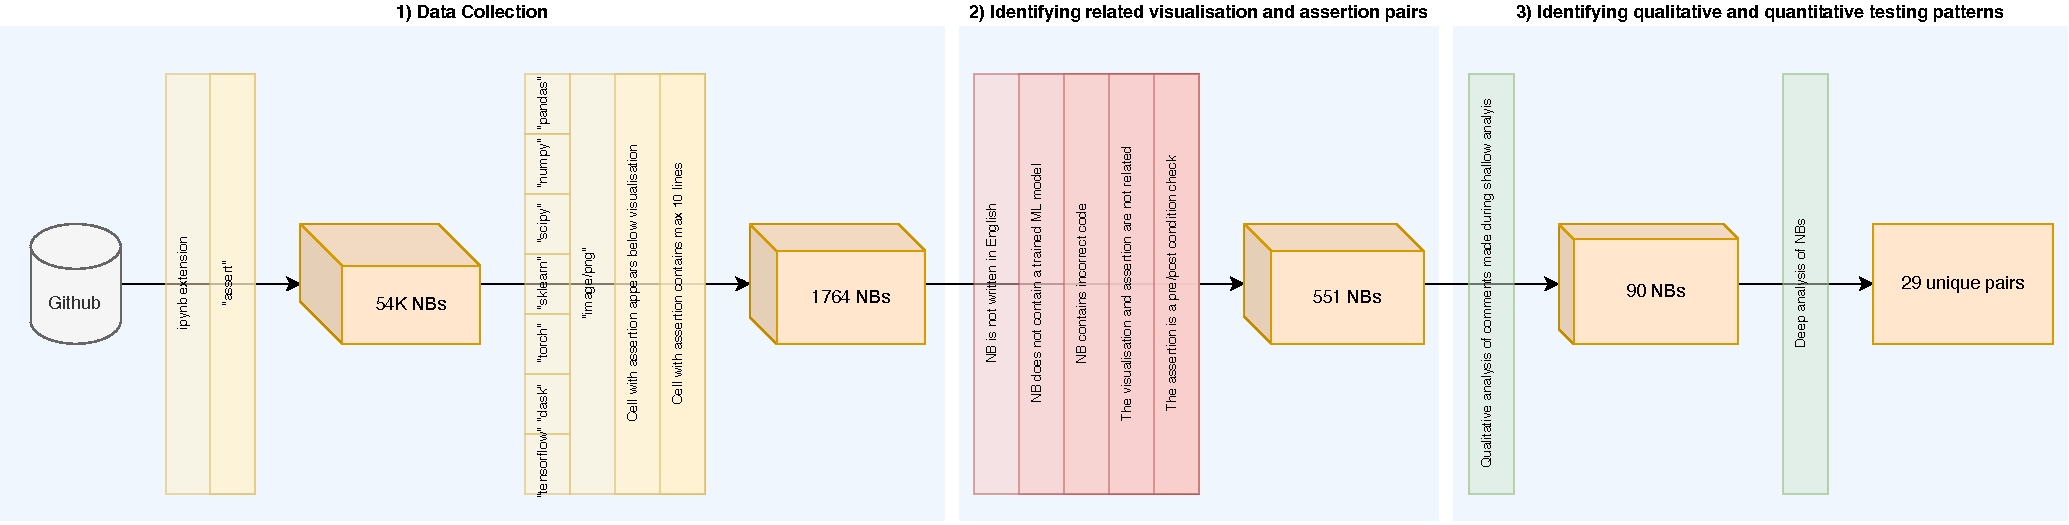
\includegraphics[width=\textwidth]{method.pdf}
  \caption{Methodology used to collect and analyse Jupyter notebooks
    in this study.}
  \label{fig:method}
\end{figure}

\subsection{Data Collection}\label{sec:data-collect}

We mined public repositories from Github to collect Jupyter notebooks that contain the keyword ``assert'' in them. We intentionally keep the search criteria on Github broad by only checking for the appropriate filetype and the presence of the ``assert'' keyword. This is because, the ``assert'' keyword is used in python to define tests. Additionally, popular python libraries which provide a testing interface (such as nose, unittest and numpy), contain the same keyword in their API. Our search criteria captures a large initial sample of $54,070$ notebooks with a variety of testing statements. Our approach also prevents the need to craft a custom search query based on an exhaustive list of keywords that appear in all python testing libraries.

We use the Github advanced search syntax~\footnote{REFME} to isolate Jupyter Notebook. This translates to the following Github search query: \texttt{filename:"Jupyter Notebooks"}. Additionally, we include the ``assert'' keyword in the search query with an \texttt{AND} operator. The final search query is as follows: \texttt{filename:"Jupyter Notebooks" AND "assert"}.

The above search query results in approximately 54K notebooks. To further reduce the sample size, we exclude notebooks that do not use popular ML libraries. We perform a string search to identify notebooks that import at least one of the ML libraries. The string patterns are derived from the python module name used in the import statements. The regex search query is as follows: \texttt{tensorflow|dask|torch|sklearn|scipy|numpy|pandas}.

We programmatically parse the JSON structure of the notebooks and represent each notebook as a pandas dataframe for further analysis. We map each cell as a row in the dataframe. For each cell, we store the \texttt{cell\_type}, the \texttt{source} of the cell and the base64 encoded PNG string, into the corresponding columns of the dataframe. We exclude notebooks that do not contain any visualisations by checking if the image column of the dataframe is empty. The internal structure of Jupyter notebooks is presented in Section~\ref{sec:nbformat}.

\begin{figure}
  \centering
  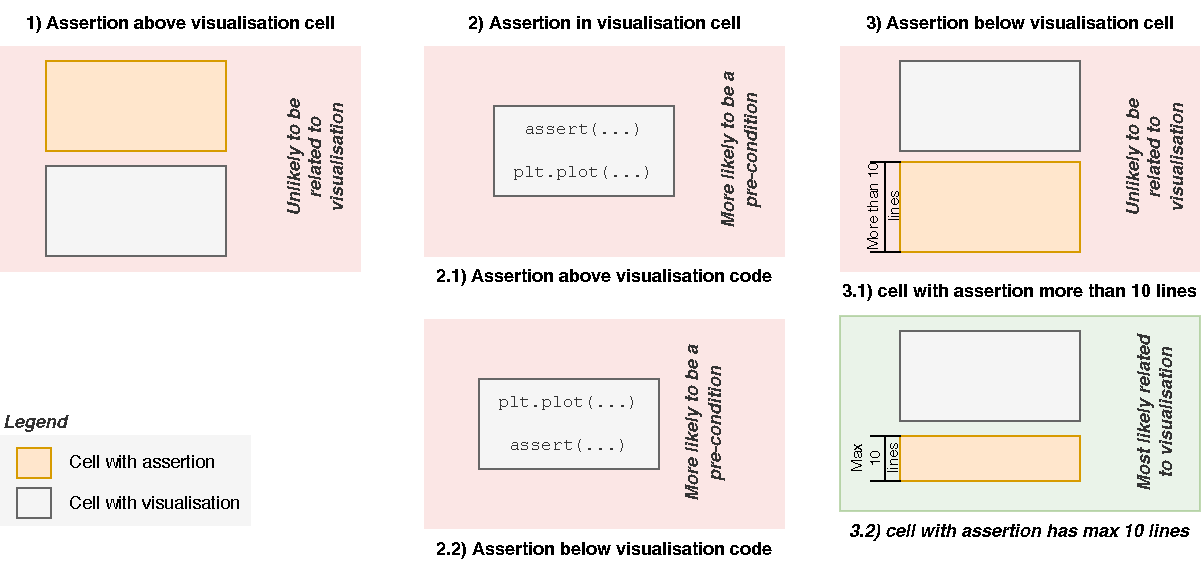
\includegraphics[width=\textwidth]{nb-structure.pdf}
  \caption{Arrangement of code cells containing assertion and
    visualisation.}
  \label{fig:cell-arrangement}
\end{figure}

For RQ1, we are interested in finding empirical evidence of visualisations and corresponding assertions used in the wild. To answer this question, we further reduce our notebook sample size by assuming a specific order in which the visualisation and assertion code cells appear in the notebooks. Figure~\ref{fig:cell-arrangement} presents a visual representation of various arrangements of code cells that may occur in notebooks. Note that the visual representation omits markdown cells since we only consider the order of code cells in our analysis. In the actual notebook however, one or more markdown cells may be present between the visualisation and assertion cells.


% TODO don't mention quantity of random sample; then we need to explain/defend this choice
We used an iterative approach to determine the effectiveness of each
filter that was used. We applied each filter in the same order as
presented in Table~\ref{tab:filters}, starting with F1. We randomly
sampled 50 notebooks from the population of notebooks obtained after
applying the filter. We then conduct the qualitative assessment
presented in Section~\ref{REFME} and observe the number of related
visualisation and assertion pairs. In each new iteration, we
progressively add the other filters and include the filter if the
number of relevant visualisation and assertion pairs increases.

As explained above, the selected arrangement of code cells was discovered by qualitatively analysing a random sample of notebooks with the code cell arrangements presented in Figure~\ref{fig:cell-arrangement}. We observed the signal-to-noise ratio for each cell arrangement. And picked the arrangement with the least signal-to-noise ratio. Table~\ref{tab:cell-arrangement} summarises our observations from the various cell arrangements.

% TODO give more examples (from our data) of what a pre/post condition check is
\begin{table}
  \centering
  \caption{Observations from random samples of notebooks with various
  cell arrangement.}
  \begin{tabular}{l p{0.4\textwidth} p{0.4\textwidth}}
    \toprule
    \emph{\textbf{ID}}&
    \emph{\textbf{Cell arrangement}} &
    \emph{\textbf{Observations}}\\
    \midrule
    1 &
    Assertion above visualisation cell &
    The assertions in this arrangement were typically not related to the visualisation below. Often, a markdown cell present between the assertion and visualisation code cells, would mark the begining of a new section in the notebook. In other cases, the assertions were typically pre-condition checks to ensure that the visualisation code would not encounter any errors. Pre-condition checks typically include checking the shape of features that are used in the visualisation. Or checking that the length of the ``x''and ``y`` features are the same to ensure a continuous line in the plot.\\
    2.1 &
    Assertion in the visualisation cell: assertion above visualisation code &
    Our observations were similar to that of arrangement 1. the assertions defined above the visualistion code were more likely to be pre-condition checks.\\
    2.2 &
    Assertion in the visualisation cell: assertion below visualisation code &
    We found several examples where the assertion was related to the visualisation. Most often however, the assertions were post-condition checks to ensure the correctness of the visualisation itself. The signal-to-noise ratio in this arrangement was also higher compared to arrangement 3.2.\\
    3.1 &
    Assertion below visualisation cell: assertion cell more than 10 lines &
    The assertions in this arrangement were frequently related to the visualisation above. In some cases, a markdown cell between the visualisation and assertion marked the begining of a new section in the notebook indicating that the visualisation and assertion were not related to each other. We also observed instances where the assertion cell defined a new class or several helper methods that were not related to the visualisation above. This motivated our decision to only flag notebooks where the assertion cell was no longer than 10 lines.\\
    3.2 &
    Assertion below visualisation cell: assertion cell has max 10 lines &
    This arrangement had the highest signal-to-noise ratio. We observed that most notebook authors followed the convension of writing their motivation for the visualisation in a markdown cell, before writing the code for the visualisation. The visualisations were often followed by another markdown cell to record the author's observations. And finally, the observations were translated to a analytical test using \texttt{``assert''} or other testing methods from external libraries.\\
    \bottomrule
  \end{tabular}
  \label{tab:cell-arrangement}
\end{table}

\subsection{Identifying Related Visualisation and Assertion Pairs}\label{sec:identify-related-pairs}

% TODO the numbers don't line up, because the annotations were not perfect. We 161 instances where I did not SELECT the notebook but also did not assign it an EC. How do we handle this?
% NOTE move the 161 with the 337, then we can say we had 500+ notebooks and we cannot analyse them all in depth...
The initial sample size of 54K notebooks from Github, was reduced to the final sample size of 1.7K after applying the filters presented in Section~\ref{sec:data-collect}. We analysed all 1.7K notebooks manually to further identify 337 notebooks that contained at least one pair of visualisation and assertions that were related to each other. Table~\ref{tab:exclusion-criteria} presents the exclusion criteria used in this phase of the analysis, along with the number of notebooks that were excluded based on each criteria.

\begin{table}
  \centering
  \caption{Exclusion criteria used during phase 2 to identify related visualisation and assertion pairs.}
  \begin{tabular}{l p{0.3\textwidth} p{0.4\textwidth} p{0.1\textwidth}}
    \toprule
    \textbf{ID} &
    \textbf{Exclusion Criteria} &
    \textbf{Rationale} &
    \textbf{Num. excluded NBs}\\
    \midrule
    \textbf{EC1} &
    Notebook not written in English &
    % TODO find a better way to phrase this?
    We excluded notebooks that were not authored in English since that is the primary language of all authors of this paper. &
    159\\
    \textbf{EC2} &
    Notebook does not contain a trained ML model &
    % TODO need to explain this better, we have notebooks with diverse python libraries; different ML models work differently so we need to understand the maths behind it.
    We excluded notebooks that did not train an ML model. We found several notebooks that were on topics related to ML such as linear algebra, optimization and loss functions to name a few. However, identifying how the visualisation and assertion pairs can be applied to a production ML system, requires a deep understanding of several python libraries and the inner workings of various ML models. This was deemed beyond the scope of this research project. &
    383\\
    \textbf{EC2} &
    Notebook contains incorrect code &
    % TODO our filter excludes NBs without images, we have to defend why this EC is still required: jupyter adds the "image/png" field regardless of error in code
    We excluded notebooks that contained incorrect code that did not produce a visualisation. We also excluded notebooks that used \texttt{assert} statements to stop execution of a code cell. &
    31\\
    \textbf{EC3} &
    % TODO is there technical terminology for what we did to identify if the visualisation & assertion are related to one another?
    % TODO I think we need a brief paragraph on how we prompted ChatGPT, this stuff probably needs to go outside of a table!
    The visualisation and assertion are not related &
    We excluded notebooks where the visualisation and assertion pairs were unrelated. We manually analyse the source code of the visualisation and the assertion to determine if they are related to one another. In some instances, the tracing was not straightforward or the code was not well written. In such cases, we used one-shot prompt engineering with ChatGPT 4.0 model to derive the link between the visualisation and the assertion. &
    440\\
    \textbf{EC4} &
    The assertion is a pre or post-condition check &
    % TODO we have to give examples of pre/post condition checks. I think this content needs to be outside of a table!
    We excluded &
    200\\
    \bottomrule
  \end{tabular}
  \label{tab:exclusion-criteria}
\end{table}

\subsection{Deeper Analysis of Notebooks}\label{sec:deep-dive}

We qualitatively assess the comments made for all notebooks during the analysis conducted in phase two of the study, as described in Section~\ref{sec:identify-related-pairs}. We perform an in-depth analysis of 90 short-listed notebooks to identify unique ML testing tasks. The in-depth analysis was conducted by reading and understanding the entire contents of the notebooks in a top-down order. During the analysis, we note several data points such as the primary objective of the notebook, the type of ML problem, the type of ML model and the type of data. We manually read and comprehend each code cell in the notebooks. When present, we also read the markdown cells above and below code cells to gain further context from the notebook author. For instance, we find that markdown cells above a visualisation cell typically motivates the need for the visualisation. A markdown cell directly below a visualisation often records the observations made by the notebook author from the visualisation.

\section{Results}\label{sec:result}
This study identified 26 patterns of testing using visualisation and assertion. This section highlights five interesting patterns in more detail. We plan to release the entire catalogue of patterns publicly in the near future.

\subsection{Decision boundary}\label{sec:svm}

% NOTE something about how the visualisation helps with interpretability of how the model is classifying the data?

% NOTE the author is using the visualisation to iteratively check/test how different kernels perform on the data; can also use it for hyper-parameter tuning?

% NOTE: visualisation can provide qualitative assessment of under/overfitting

% NOTE: better assertion: perhaps on the support vectors?

\begin{figure}
  \subcaptionbox{Visualisation of the decision boundary of a SVM with a linear kernel.\label{fig:svm-linear}}{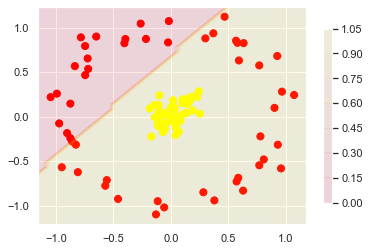
\includegraphics[width=0.45\linewidth]{../catalogue/select-04-linear.png}}
  \hfill
  \subcaptionbox{Visualisation of the decision boundary of a SVM with a RBF kernel.\label{fig:svm-rbf}}{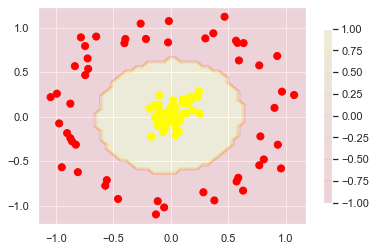
\includegraphics[width=0.45\linewidth]{../catalogue/select-04-rbf.png}}
  \caption{Visualisation of the decision boundary of a SVM trained using different kernels.}
  \label{fig:svm}
\end{figure}

\begin{lstlisting}[language=Python]
assert accuracy_score(y_test, pred) > 0.95
\end{lstlisting}
\captionof{lstlisting}{Assertion on the accuracy of the ML model.}\label{lst:svm}

Figures~\ref{fig:svm} presents visualisations obtained from a notebook that performs binary classification using Support Vector Machines (SVM). The model is trained on the \texttt{make\_circles}~\footnote{REFME} dataset obtained from scikit-learn~\footnote{REFME}. The visualisations show the two classes present in the training set, and the decision boundary of the model when trained first using a linear kernel (Figure~\ref{fig:svm-linear}) and later with a RBF kernel (Figure~\ref{fig:svm-rbf}). Listing~\ref{lst:svm} shows the corresponding assertion that was defined below the visualisations. The assertion checks if the model accuracy is above a threshold specified by the author of the notebook.

Visualising the decision boundary of a SVM provides a visual understanding of how the model is performing for a given dataset. Mis-classified examples can be seen on the wrong side of the decision boundary. The visualisation can also be used to check if the model is overfitting or underfitting the data. For instance, in Figure~\ref{fig:svm-linear} we observe that the model is underfitting since a linear kernel too simply for the underlying data.

\subsection{Input Image, \texttt{predict\_proba}}

\begin{figure}
  \subcaptionbox{Random input image of a football from the test set.\label{fig:football}}{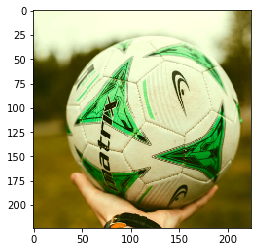
\includegraphics[width=0.45\linewidth]{../catalogue/select-35a.png}}
  \hfill
  \subcaptionbox{Random input image of tennis balls from the test set.\label{fig:tennisball}}{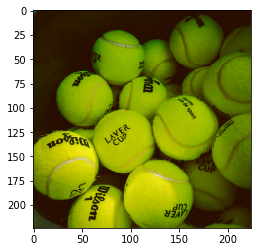
\includegraphics[width=0.45\linewidth]{../catalogue/select-35b.png}}
  \caption{Visualisation of random input images for a pre-trained image classifier.}
  \label{fig:balls}
\end{figure}

\begin{minipage}{0.45\textwidth}
  \begin{lstlisting}[language=Python]
np.testing.assert_almost_equal(pred_proba, 2.0355723e-05, decimal=3)
  \end{lstlisting}
  \captionof{lstlisting}{Assertion to check if the probability estimate of the model is close to the specified value. The input image is of a football. Since the model is trained to detect tennis balls, the specified value is very small.}
  \label{lst:football}
\end{minipage}
\hfill
\begin{minipage}{0.45\textwidth}
  \begin{lstlisting}[language=Python]
np.testing.assert_almost_equal(pred_proba, 0.9988895, decimal=3)
  \end{lstlisting}
  \captionof{lstlisting}{Assertion to check if the probability estimate of the model is close to the specified value. Compared to Figure~\ref{fig:football}, the specified value is much higher, since the input image is of tennis balls.}
  \label{lst:tennisball}
\end{minipage}

Figure~\ref{fig:balls} presents visualisations obtained from a notebook that uses a pre-trained image classifier from GluonCV library~\footnote{https://cv.gluon.ai}, to identify images that contain tennis balls.The visualisations are of two random input images, one from each class in the dataset. Listing~\ref{lst:football} presents the assertion related to Figure~\ref{fig:football}. The assertion checks if the probability estimate of the model for the given input image, is close to the specified value with a precision of up to three decimal places. Since the model is trained to detect tennis ball, and the input image contains a footbal, the specified probability estimate is very low. In contrast, Listing~\ref{lst:tennisball} specifies a much higher probability estimate since the input image contains tennis balls.

The above testing technique can be used to spot-check a few hand-picked examples of edge cases or adversarial examples which the model may find difficult to classify. The technique can also be generalized by constructing a large dataset containing all the edge cases that the develop may wish to check. And the assertion can be called on the probability estimate for image.

% NOTE when working with images, we tend to see that the input image is visualised (so human can manually validate), something to do with expensive labelling?
% NOTE is this a good pattern? this test does not generalise across all possible input images?

\subsection{Normality}\label{sec:normal}

\begin{minipage}{0.45\textwidth}
  \begin{lstlisting}[language=Python]
for feature in range(data_transformed.shape[1]):
  assert kstest(data_transformed[:, feature], 'norm').statistic < 1e-2
  \end{lstlisting}
  \captionof{lstlisting}{Assertion to check that each feature in a dataset is normal. The distribution of each feature is compared to that of a normal distribution using the Kolmogorov-Smirnov test for goodness of fit from the scipy library.}
  \label{lst:kstest}
\end{minipage}
\hfill
\begin{minipage}{0.45\textwidth}
  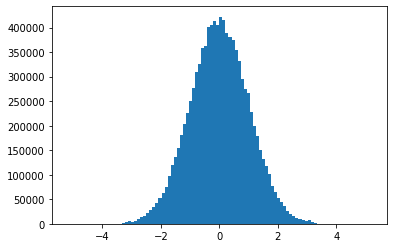
\includegraphics[width=\linewidth]{../catalogue/select-152a.png}
  \captionof{figure}{Visualisation of the distribution of a feature from the dataset.}
  \label{fig:kstest}
\end{minipage}

\subsection{Coefficient of Determination}

Figure~\ref{fig:r2} shows a visualisation obtained from a notebook that trains a RNN to predict the levels of Nitrogen Dioxide ($NO_2$) in the next 24 hour window. The model is trained using time-series data consisting of historical readings of $NO_2$ and meteorological data such as temparate, humidity, wind speed, and such. The visualisation shows a scatterplot of the real and predicted values of $NO_2$ from the test set. The scatterplot shows a linear relationship between the ground truth and predictions indicating that the model learned something during training. However, the spread of the points is wide indicating that it can be improved with more fine tuning. Listing~\ref{lst:r2} presents the corresponding analytical test which was defined below Figure~\ref{fig:r2}. The Coefficient of Determination ($R^2$) is calculated using the \texttt{r2\_score} method from scikit-learn. The assertion checks that the $R^2$ is higher than a specified threshold.

\begin{minipage}{0.45\textwidth}
  \begin{lstlisting}[language=Python]
r2_gru = r2_score(y_test, y_pred)
assert r2_gru > 0.6
  \end{lstlisting}
  \captionof{lstlisting}{Assertion to check that the Coefficient of Determination ($R^2$) is higer than the specified threshold.}
  \label{lst:r2}
\end{minipage}
\hfill
\begin{minipage}{0.45\textwidth}
  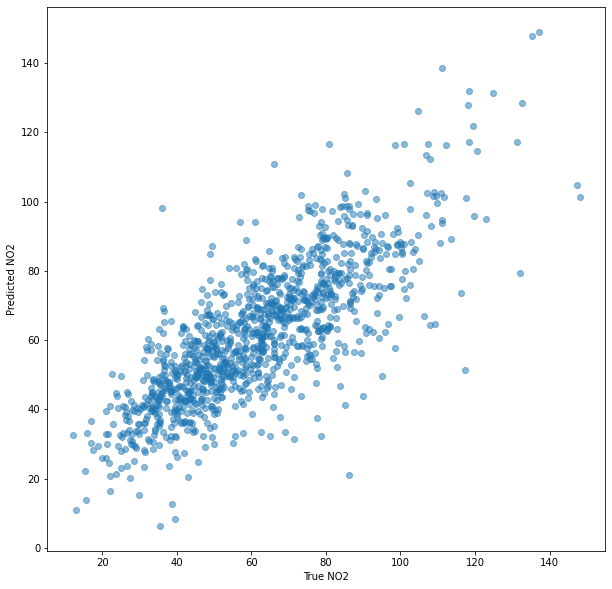
\includegraphics[width=\linewidth]{../catalogue/select-332a.png}
  \captionof{figure}{Scatterplot of the actual and predicted labels of a dataset. The visualisation shows that there is a linear relationship between the true and predicted labels.}
  \label{fig:r2}
\end{minipage}

\subsection{Normalization}

\begin{minipage}{0.45\textwidth}
  \begin{lstlisting}[language=Python]
assert normalized_data[normalized_data.argmax()] < 10
assert normalized_data[normalized_data.argmin()] > -7
  \end{lstlisting}
  \captionof{lstlisting}{Assertion to check that the min and max of a feature fall within specified thresholds derived from the visualisation presented in Figure~\ref{fig:normal}.}
  \label{lst:normal}
\end{minipage}
\hfill
\begin{minipage}{0.45\textwidth}
  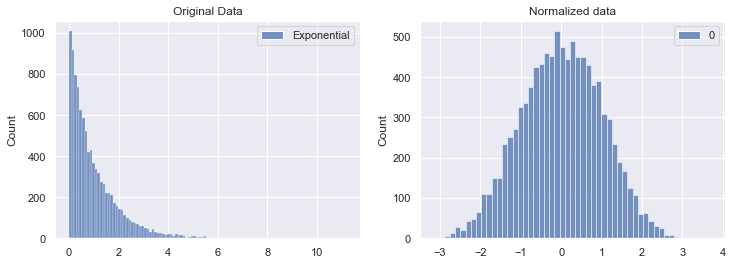
\includegraphics[width=\linewidth]{../catalogue/select-65b.png}
  \captionof{figure}{Histogram showing the distribution of a feature before and after normalisation.}
  \label{fig:normal}
\end{minipage}

\section{Discussion}\label{sec:discuss}

% NOTE comment on the over-whelming presence of magic thresholds in ML testing! where are authors getting these numbers from? link this to requirements engineering?

% NOTE comment on the anti-patterns in testing that we observe in the 5 patterns presented

% NOTE link the qualitative and quantitative testing to the ML lifecycle: how some tests will let practitioner know when something changes

% NOTE comment on evolution? we have to look at the entire lifecycle of a visualisation: notebooks are run iteratively?

\subsection{Evolution and Provenance of Visualisations}\label{sec:evolution}
% NOTE ML development is iterative, visualisations are compared against one another, to qualitatively validate performance/different strategies of model performance? It will be an interesting direction to explore how visualisations evolve?

\subsection{Something about magic thresholds}\label{sec:magic-threshold}
% NOTE we observe that most analytical test translates to comparing a value against a threshold; this indicates the open challenges in ML testing; either we don't yet know how to translate analytical tests from visualisations or we cannot do this in the first place and we must use a hybrid approach?

\subsection{Warning System}\label{sec:drift}
% NOTE with the assertions, the implicit expectations are translated to explicit expectations. Which will fail if the expectations are no longer satisfied

\section{Threats to Validity}\label{sec:threats}
% defend use of github as source for notebooks:
% - why did kaggle not work (refer to notes)
% - why did the existing replication packages not work?

% motivation for keeping the search on github broad:
% - not only does it pick up python assert statements, but also flags
% - notebooks that use other testing libraries or modules that provide a
% - testing interface. This is a good compromise between doing an
% - exhaustive search of all testing method names in the python
% - ecosystem and then doing a search for each of those patterns
\section{Conclusion}\label{sec:conclude}

\bibliographystyle{ACM-Reference-Format}
\bibliography{bibliography}
\end{document}

